\chapter{Physics Background} \label{ch:2}

At the most basic level, a plasma is a state of matter that largely consists of charged particles (rather than neutral particles). Typically, this is achieved by heating a solid, liquid, or gas so much that the constituent atoms achieve a sufficient level of ionization. Francis Chen, author of a prominent plasma physics textbook \cite{Chen_2015_Plasma}, describes a plasma as

\begin{quote}
	a \emph{quasineutral} gas of charged and neutral particles which exhibits \emph{collective behavior}
\end{quote}
In this chapter, laser fields and the physics of charged particles oscillating in them will be overviewed to better understand the plasmas produced from laser-matter interactions. Plasma properties and their relation to quasineutrality and collective behavior will be discussed. Then, ion-acceleration will be explained in the context of laser-plasma interactions.
%\begin{table}
%\begin{center}
%\begin{tabular}{lll}
%\hline
%\\[3pt]
%Alphabet Character & Vowel & Number \\[3pt]
%\hline
%\\[3pt]
%A & Yes & 1 \\
%B & No & 2 \\
%C & No & 3 \\[3pt]
%\hline
%\end{tabular}
%\label{tbl3}
%\caption{Another Table}
%\end{center}
%\end{table}

\section{Electric Fields}


\subsection{Gaussian Laser}
In order to heat up a material with a laser efficiently, the energy would ideally be concentrated to a small point. Lasers are a coherent source of light that can be focused to narrow beams. The intended output of many lasers is the fundamental transverse electromagnetic mode \cite{Zangwill_2012} (TEM$_{00}$) described by the following electric field

\begin{equation}
	\vec{E}(r, x) = \hat{y} E_0  \frac{w_0}{w(x)} \exp \left( - \frac{r^2}{w(x)^2} \right) \cos \left(k x - \omega t - \arctan \left(\frac{x}{x_R}\right) + \frac{k r^2}{2 R(x)}\right) \label{eq:gaussian_beam}
\end{equation}
where $\hat{x}$ is the propagation direction, $\hat{y}$ is the polarization direction, and $r = \sqrt{y^2 + z^2}$ is the radial distance away from the laser axis. The radius of curvature $R(x)$ is inversely related to how strongly the wavefronts are curved and is infinity at $x=0$ and minimum at $x=x_R$. The guoy phase $\arctan(x/x_R)$ is an observed phase of $\pi$ that is continuously picked up as the beam propagates from $x=-\infty \rightarrow x=+\infty$. Additionally, the beam radius $w$ is expressed as

\begin{equation}
	w(z) = w_0 \sqrt{1 + (x/x_R)^2} \label{eq:beam_radius}
\end{equation}  
and has a minimum value at the \emph{beam waist} $w(0) \equiv w_0$ at the focal position of the laser. The length scale over which the beam can propagate without diverging significantly is the \emph{Rayleigh range} $x_R \equiv \frac{\pi w_0^2}{\lambda}$. A beam with these properties is usually referred to as a gaussian beam\footnote{I have googled (actually bing'd unfortunately) more times than I can count ``gaussian beam wikipedia'' over the course of my studies.} and is depicted in \autoref{fig:gaussian_beam}.

\begin{figure}
	\centering
	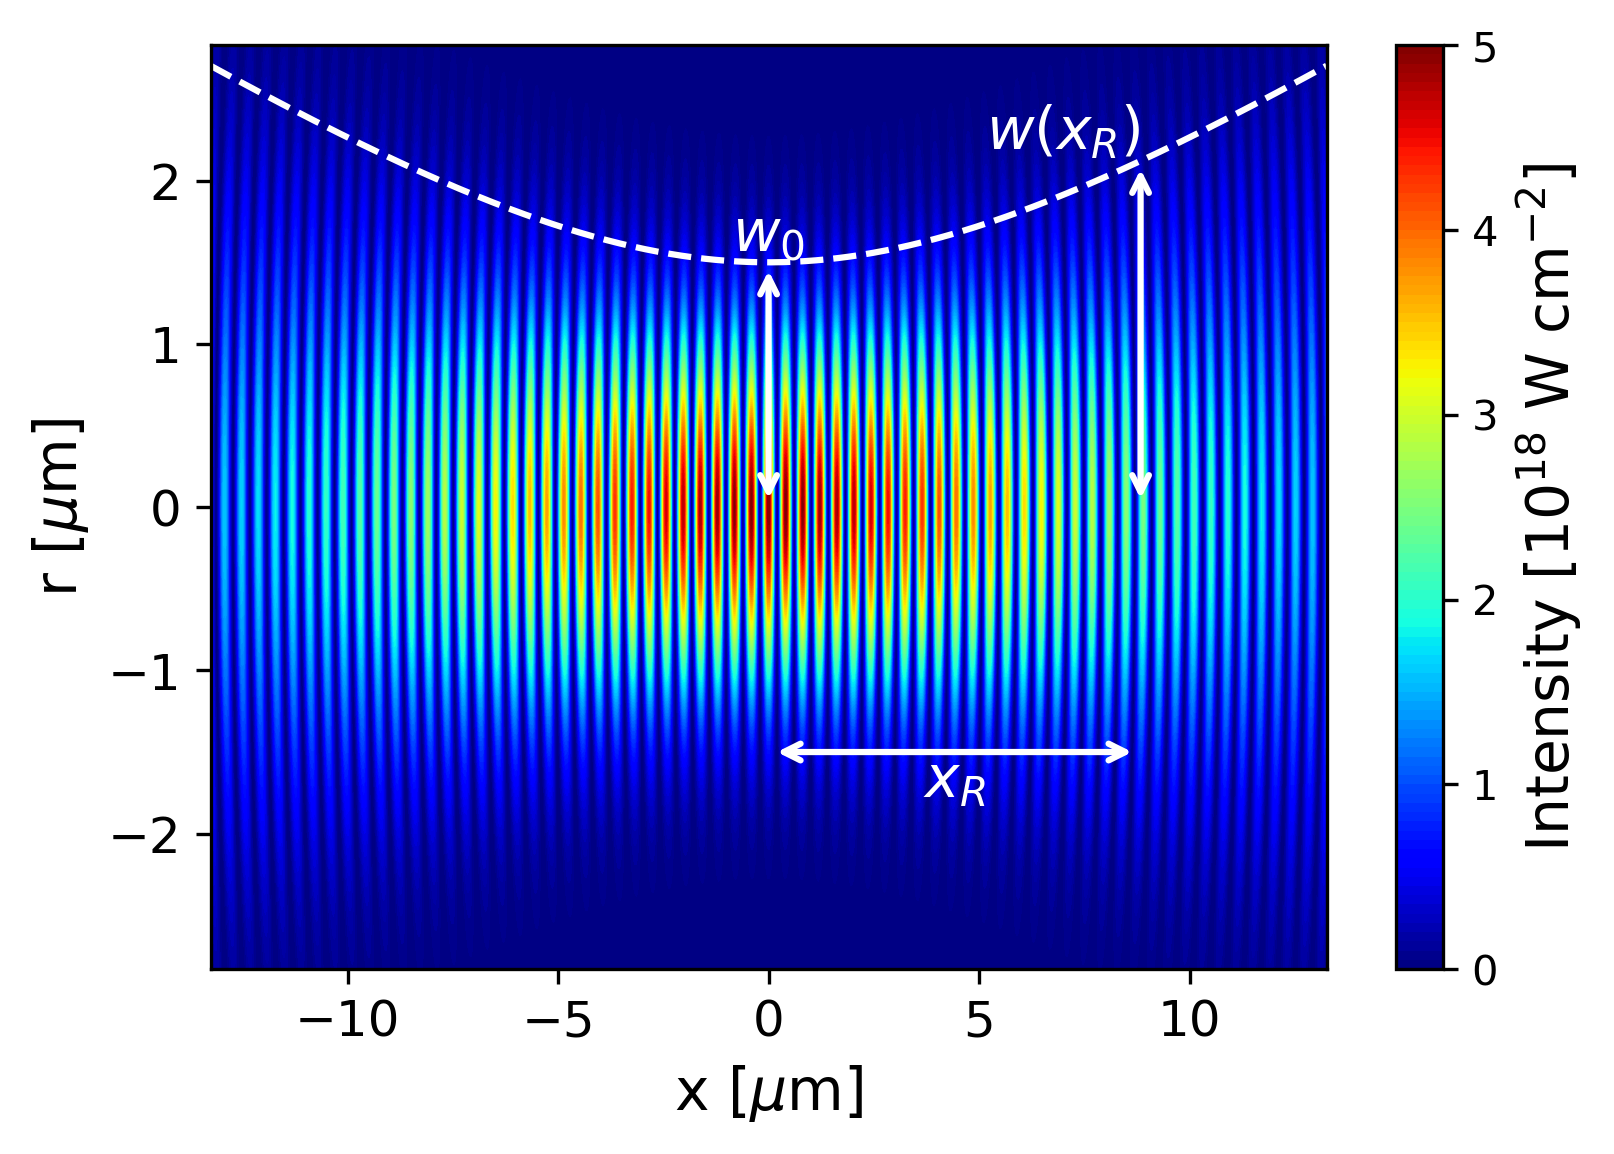
\includegraphics[width=0.75\linewidth]{planning/images/gaussian_beam.png}
	\caption{The intensity profile of a gaussian beam with laser parameters seen in the Extreme Light Laboratory at Wright-Patterson Air Force Base ($\lambda = 0.8 \mu$m, $I_0=\SI{5e18}{\watt \per \centi \meter \squared}$, $w_0 = \SI{1.5}{\micro \meter}$, $\tau_\text{FWHM}=40$fs). The beam radii $w_0$ and $w(x_R)$ are displayed in addition to the rayleigh range $x_R$.}
	\label{fig:gaussian_beam}
\end{figure}

The peak intensity is related to the electric field by $I_0 = \frac{1}{2} \epsilon_0 c E_0^2$ and \cref{eq:gaussian_beam} shows that the intensity decays as $I(x, r) = I_0 (w_0 / w(x))^2 \exp(-2 r^2 / w(x)^2)$ with increasing $r$ and $x$. If we integrate this intensity distribution over the entire $y-z$ plane (at $x=0$), we obtain the peak power $P_0 = \frac{\pi \omega_0^2}{2} I_0$. Furthermore, we can integrate the power over the pulse duration (assuming a $\sin^2(t)$ envelope\footnote{As with most things in physics, when there's an oscillating or pulsed quantity, it typically follows a sinusoidal distribution. The pulse envelope is related to the intensity which is proportional to the square of the electric field. It is possible for the pulse shape to be slightly different (like a gaussian function), but the expressions for energy and pulse \gls{FWHM} do not change significantly.}) to obtain the total energy in the pulse 

\begin{equation}
	E = \frac{\pi \omega_0^2}{2} I_0 \tau_\text{fwhm} \label{eq:gaussian_beam_energy}
\end{equation}
where $\tau_\text{fwhm}$ is the full-width half-max (half the pulse duration for a $\sin^2(t)$ pulse envelope). 

\subsection{Single Particle Motions}

Electromagnetism is governed by Maxwell's equations which describe the allowed wave-like solutions for electric and magnetic fields in both matter and vacuum. The most relevant equation in this section is Gauss' Law or Poisson's Equation which can be expressed as 

\begin{equation}
	- \nabla^2 \phi = \nabla \cdot \vec{E} \equiv \frac{\rho}{\epsilon_0} \label{eq:poisson}
\end{equation}
which relates the electrostatic potential $\phi$ or electric field $E$ to the charge density $\rho$. This equation highlights how electric fields are directed radially outward from positive charges and inward towards negative charges. The motion of an electron in the influence of an electric field $E$ or magnetic field $B$ is given by the \emph{Lorentz force} $F_L$

\begin{equation}
	F_L \equiv -e (\vec{E} + \vec{v} \times \vec{B}) \label{eq:lorentz}
\end{equation}

\subsubsection{Quiver Energy}
To gain intuition about some quantities of interest for laser-matter interactions, let's consider the simple problem of an electron of charge $-e$ governed by \cref{eq:lorentz} with a negligible magnetic field $B$. Additionally, only consider 1D motion in the oscillating field $E = E_0 \cos(\omega t)$ for a laser field of frequency $\omega$ (which can be considered a simplification of \autoref{eq:gaussian_beam} when $\lvert x \rvert \ll x_R$ and $r \ll w_0$). Then, the equation of motion is

\begin{equation}
	\frac{d v}{d t} = - \frac{e E_0}{m} \cos(\omega t)
\end{equation}
We can integrate this equation to obtain the velocity and position as a function of time (assuming $x_0 = v_0 = 0$)

\begin{align}
	v(t) &= - v_\text{osc} \sin(\omega t) \label{eq:v(t)} \\
	x(t) &= \frac{v_\text{osc}}{\omega} [\cos(\omega t) - 1] \label{eq:x(t)}
\end{align}
where $v_\text{osc} \equiv (e E_0) / (m \omega)$ is defined as the \emph{quiver velocity}. From \autoref{eq:v(t)}, we can calculate the kinetic energy gained by an electron as $U_p \equiv \frac{1}{2} m \langle v^2 \rangle = \frac{1}{4} m v_\text{osc}^2$ which is known as the \emph{ponderomotive potential (energy)}. This energy represents the cycle-averaged quiver energy of an electron in an electromagnetic field. A more commonly used term is the dimensionless \emph{normalized vector potential} $a_0$ which is closely related to the quiver velocity

\begin{equation}
	a_0 \equiv v_\text{osc} / c = \frac{e E_0}{m \omega c} \label{eq:a0}
\end{equation}
Ultra-intense laser-matter interactions involve relativistic electrons\footnote{Although $v_\text{osc}$ can be greater than $c$, relativistic electrons are still limited by the speed of light.} which are produced when $a_0 \gtrsim 1$. In terms of the field, $a_0 \sim 1$ corresponds to a peak electric field $E_0 = \frac{2 \pi m c^2}{e \lambda} \simeq \SI{4}{\tera \volt \per \meter}$ (for a $\lambda \approx \SI{1}{\micro \meter}$ wavelength). For this electric field, the peak intensity is $I_0 = \frac{1}{2} c \epsilon_0 E_0^2 \simeq \SI{2e18}{\watt \per \centi \meter \squared}$ for this electric field. Consequently, the threshold for relativistic interactions is commonly understood as $I_0 \gtrsim \SI{1e18}{\watt \per \centi \meter \squared}$ for typical micron wavelength lasers. 

\subsubsection{Ponderomotive Force}
The above approach yields some important scales for laser-matter interactions, but only describes the interaction of a plane wave that is spatially homogeneous. A real laser field would be spatially inhomogeneous and we can express $E(x) \approx E_0 + x E_0'(x)$ (where the prime denotes the derivative with respect to $x$) to first order. This modifies the equation of motion as 

\begin{equation}
	\frac{d v}{d t} = - \frac{e E_0}{m} \cos(\omega t) - \frac{e E_0'}{m} \cos(\omega t)[ \frac{v_\text{osc}}{\omega}(\cos(\omega t) - 1)]
\end{equation}
where we have inserted the expression for x from \cref{eq:x(t)} which should be approximately true for small $x$. This equation can be simplified and separated into oscillating and non-oscillating components as

% should maybe cite arefiev notes, not sure how, because I can't find it online.
\begin{equation}
	\frac{d v}{d t} = - \frac{e E_0}{m} [\cos(\omega t)(1 - \frac{E_0' v_\text{osc}}{e_0 \omega}) + \frac{E_0' v_\text{osc}}{2 \omega E_0} \cos(2 \omega t)] - \frac{e E_0' v_\text{osc}}{2 m \omega}
\end{equation}
Over many cycles, the oscillating components will average out to zero and the remaining term is given by $\langle F_p \rangle = m \frac{d v}{d t} = - \frac{e E_0' v_\text{osc}}{2 m \omega}$ and is called the \emph{ponderomotive force}. We can generalize this to 3D and express this time-averaged force in several different, equivalent ways

\begin{equation}
	\langle F_p \rangle = - \frac{e^2}{2 m \omega^2} \lvert E_0 \rvert \nabla E_0 = - \frac{m c^2}{4} \nabla(a_0^2) = - \nabla U_p \label{eq:pond_force}
\end{equation}
where 
\begin{equation}
	U_p = \frac{e^2 E_0^2}{4 m \omega^2} = \frac{1}{4} m v_\text{osc}^2 \label{eq:pond_potential}
\end{equation}
is the ponderomotive potential energy introduced earlier. The ponderomotive force is an important mechanism in the absorption of laser energy by electrons which will be expanded upon in \cref{sec:absorption}.

\section{Plasma Physics}
The quasi-neutrality condition reflects the fact that a plasma is charge neutral throughout its volume in a similar way to an ideal conductor: mobile electrons will reorganize themselves in the presence of an external electric field to maintain zero field (or constant  potential). The simplest plasma description will assume the ions are immobile (due to being much heavier than the electrons) and can be treated as a constant neutralizing background density $n_i$ for the electrons of density $n_{e,0} = Z n_i$ (for a plasma with atomic number $Z$).

\begin{figure}
	\centering
	\includegraphics[width=0.75\linewidth]{planning/images/plasma_oscillation.PNG}
	\caption{An initially charge-neutral plasma is depicted on the left. On the right, the electrons are displaced by a distance $x$ creating a charge separation and electric field akin to a parallel-plate capacitor directed towards the right. Adapted from Smith \cite{Smith_2020_Thesis}.}
	\label{fig:plasma_oscillation}
\end{figure}

\subsection{Plasma Electron Oscillations}
A simple example can be illustrated by \cref{fig:plasma_oscillation} which shows a sheet of negative charge density $-\sigma = -e n_e x$ displaced to the right a small distance $x$. The region in the bulk of the plasma will experience a force from the parallel plate ``capacitor'' fields directed to the left.

\begin{equation}
	F = m \frac{d^2 x}{d t^2} = - e \frac{e n_e x}{\epsilon_0}
\end{equation}
which has the form of a restoring force that brings the charge imbalance back to the center of the plasma. This oscillatory motion has an associated frequency 

\begin{equation}
	\omega_{p,e} = \sqrt{\frac{n_e e^2}{m_e \epsilon_0}} \label{eq:omegape}
\end{equation}
that gives the timescale for electron motion in the plasma. This characteristic frequency shows why plasmas support collective motion (in opposition to a neutral gas in which collisions between individual particles only happen). To get a feeling for this timescale, let's assume a somewhat typical electron density \SI{1e29}{\per \meter \cubed} in an ionized solid or liquid to yield a timescale of $\omega_{p,e}^{-1} \simeq \SI{0.1}{\femto \second}$.

Naturally (without externally imposed forces), these fluctuations in charge could be caused by thermal motions of electrons with a characteristic speed $v_{th}$ 

\begin{equation}
	v_{th} = \sqrt{\frac{k_B T_e}{m}} \label{eq:vthermal}
\end{equation}
Due to the strong restoring force from the charge separation, the electrons can only move a short distance $\lambda_D$, called the Debye length, out of equilibrium in this timescale. We can estimate this length by equating $v_{th} = \lambda_D / t \simeq \lambda_D \omega_{p,e}$ and solve for $\lambda_D$.

\begin{equation}
	\lambda_D = \frac{v_{th}}{\omega_{p,e}} = \sqrt{\frac{\epsilon_0 k_B T_e}{n_e e^2}} \label{eq:debye}
\end{equation} 
Physically, $\lambda_D$ gives a length scale over which the electrostatic force persists in a plasma. Within a distance $\lambda_D$ from some perturbation, charges will feel a force, and outside this distance, the charges will be completely shielded like that of an ideal conductor. 

\subsection{Fluid Model}
This description of a plasma as a sea of electrons with collective motion that allows wave-like motions naturally lends itself toward a fluid model. The first component of this model stems from \cref{eq:lorentz} whose explicit time and space dependence can be expressed through

\begin{equation}
\frac{d p}{d t} = m \left( \frac{\partial v}{\partial x} \frac{\partial x}{\partial t} + \frac{\partial v}{\partial t} \right) = m \left(\frac{\partial v}{\partial t} + v \frac{\partial v}{\partial x} \right)
\end{equation}
which just considers one spatial dimension for simplicity. The second component of this model is simply related to the pressure gradient from thermal motions. Particles tend to migrate from areas of higher pressure to lower pressure, where the thermal pressure is given by the ideal gas law equation of state $p = n_e k_B T_e$. Consequently, the equation of motion should have a term that is opposite to the pressure gradient direction (i.e. $- \nabla p$). Combining these two components together in a generalized 3D equation results in

\begin{equation}
	m n_e \left(\frac{\partial \vec{u}}{\partial t} + (\vec{u} \cdot \nabla) \vec{u} \right) = -e n_e (\vec{E} + \vec{u} \times \vec{B}) - \nabla p \label{eq:fluid}
\end{equation}
where we've changed the single particle velocity $\vec{v}$ to the fluid velocity $\vec{u}$ and multiplied by the electron density $n_e$ to ensure correct units with the pressure gradient term. 

Using \autoref{eq:fluid}, we can determine the spatial extent of the electric field caused by a charge imbalance in a plasma by making some simplifications. Assuming radial symmetry where the fluid velocity $u = 0$, magnetic field $B$ is negligible, and the temperature is constant (isothermal), \autoref{eq:fluid} reduces to

\begin{equation}
	n_e e E = - k_B T_e \frac{\partial n_e}{\partial r}
\end{equation}
and by relating the electric field to the potential $E = - \frac{dV}{dx}$, this equation can be integrated from $n_{e,0} \rightarrow n_e$ and $0 \rightarrow \phi$ to obtain 

\begin{equation}
	n_e = n_{e,0} \exp \left(\frac{e \phi}{k_B T_e} \right) \label{eq:boltzmann}
\end{equation}
which is referred to as the \emph{Boltzmann relation} for electrons \cite{Chen_2015_Plasma}. We can get an approximate solution to this equation when the potential $\phi$ is only slightly larger than the equilibrium $\phi=0$, which can be found when $e \phi \ll k_B T_e$. Then, the density can be Taylor expanded to obtain 

\begin{equation}
	n_e \approx n_{e,0} \left(1 + \frac{e \phi}{k_B T_e} \right)
\end{equation} 
and if we assume a fully ionized plasma with immobile ions of charge $Z$, the density of ions satisfies $n_{e,0} = Z n_i$ and \cref{eq:poisson} becomes 

\begin{equation}
	\epsilon_0 \nabla^2 \phi = - e n_{e,0} + e n_e = e n_{e,0} \left(1 + \frac{e \phi}{k_B T_e} - 1 \right) = \frac{e^2 n_{e,0} \phi}{k_B T_e}
\end{equation}
This equation admits solutions of an exponentially decaying potential

\begin{equation}
	\phi(r) = \frac{Q}{r} \exp \left(-\frac{r}{\lambda_{D}} \right) \label{eq:shielding}
\end{equation}
where $\lambda_D = \sqrt{\frac{\epsilon_0 k_B T_e}{n_{e,0} e^2}}$ is the Debye length from \cref{eq:debye}. A visualization of the decaying potential from \cref{eq:shielding} is shown in \cref{fig:debye}. Looking at the center panel, we can see the potential drop off much more quickly than the left panel's potential. The exponentially decaying potential is a feature of plasmas and highlights the ability of plasma electrons to shield fields in a distance $\lambda_D$. 

\begin{figure}
	\centering 
	\includegraphics[width=\linewidth]{planning/images/debye_length.png}
	\caption{Visualization of the electric potential as a function of radial distance away from a positive point charge at the origin in three scenarios: vacuum (left), plasma (center), ideal conductor (right). Brighter colors show a higher value of $\phi$. In the center panel, the debye length $\lambda_D$ is shown.}
	\label{fig:debye}
\end{figure}

\subsection{Plasma Conditions}
Putting all this together, we can define several conditions that are characteristic of plasmas \cite{Chen_2015_Plasma}. Quasi-neutrality means that the bulk of the plasma is overall charge neutral, with non-neutral regions generally falling within $\lambda_D$ of some charge imbalance. Notable exceptions to quasi-neutrality are charged particle beams in ultraintense laser experiments which typically exist on a timescale shorter than the time it takes for the coulomb repulsion to blow the plasma apart. If $L$ is the length scale of the system in which the plasma resides, we require that $\lambda_D \ll L$. However, this condition is not sufficient because an ideal conductor has $\lambda_D = 0$ but is not a plasma due to the absence of collective behavior. Collective behavior can be accounted for by requiring enough electrons $N_D$ within a spherical volume of radius $\lambda_D$. The corresponding equation is $N_D = n_e (\frac{4}{3} \pi \lambda_D^3) \gg 1$. The final condition is that electrostatic interactions should dominate over collisions because the collective behavior (e.g. plasma oscillations) originates from the electrostatic forces. This means that the period of oscillations ($\omega_{p,e}^{-1}$) should be less than the mean time between collisions. 

\section{Absorption of Energy} \label{sec:absorption}

In order for a laser to couple energy to the plasma electrons, some absorption mechanism needs to take place. The most obvious way that electrons can gain energy is through collisions with other energetic electrons and ions. However, the collision frequency is known to get smaller as the temperature goes up \cite{Gibbon_2005_Plasma}, so much so that plasmas can usually be treated as collisionless for ultra-intense laser experiments. Below, some of the most common known absorption (heating) mechanisms are summarized.

\subsection{Critical Density} \label{sec:critical_density}
First, we will look at how the electric field from an oscillating electric field penetrates a plasma. Using \cref{eq:faraday,eq:ampere} combined with the vector identity $\nabla \times (\nabla \times \vec{E}) = \nabla(\nabla \cdot \vec{E}) - \nabla^2 \vec{E}$ \cite{Zangwill_2012}, we can solve for the vector wave equation in terms of only $\vec{E}$. 

\begin{equation}
	\left(\nabla^2 - \frac{1}{c^2} \frac{\partial^2}{\partial t^2} \right) \vec{E} = \mu_0 \frac{\partial \vec{J}}{\partial t} + \nabla(\nabla \cdot \vec{E}) \label{eq:vectorwave}
\end{equation}
We can look for solutions of $\vec{E} = E(x) \cos(\omega t) \hat{x}$ that vary spatially only in the x direction. We assume $E(0)$ is the amplitude of the electric field at the boundary between vacuum $x < 0$ and matter $x > 0$ and wish to understand the form of $E(x)$ when $x > 0$. To proceed, the current density can be related to the drift velocity \cite{Macchi_2013_Plasma} by $J = -n_e e u$ where $u$ is the electron fluid velocity that satisfies \cref{eq:fluid}. Ignoring $B$ and thermal pressure, this relationship becomes 

\begin{equation}
	\frac{\partial \vec{J}}{\partial t} = \frac{n_e e^2}{m} \vec{E} = \omega_p^2 \epsilon_0 \vec{E}
\end{equation}
using \cref{eq:omegape} which can be combined with \cref{eq:vectorwave} to obtain a differential equation for the electric field

\begin{equation}
	\left( \nabla^2 + \frac{\omega^2}{c^2}(1 - \frac{\omega_p^2}{\omega^2}) \right) \vec{E} = 0
\end{equation}
By just focusing on the x-dependence, we can simplify this equation to 

\begin{equation}
	\frac{d^2 E}{d x^2} = \frac{1}{l_s^2}  E
\end{equation}
where $l_s^2 \equiv \frac{c^2}{\omega^2 - \omega_p^2}$ defines the \emph{skin depth} $l_s$. In the case where $\omega < \omega_p$, $l_s^2$ is negative and the solution has a sinusoidal dependence

\begin{equation}
	E(x) = E(0) \cos \left( \frac{x}{l_s} \right)
\end{equation}
On the other hand, when $\omega > \omega_p$, $l_s^2$ is positive and the solution has an exponential dependence

\begin{equation}
	E(x) = E(0) \exp \left(-\frac{x}{l_s} \right)
\end{equation}
This ``evanescent'' behavior when $\omega > \omega_p$ occurs because the electrons cannot respond fast enough to the higher frequency $\omega$. Since the field cannot propagate effectively for $x > 0$, the plasma ends up reflecting a significant portion of the light. The critical density $n_c$ is defined as the electron density where $\omega = \omega_{p}$. Using \cref{eq:omegape}, this can be expressed as

\begin{equation}
	n_c \equiv \frac{m \epsilon_0}{e^2} \omega^2 \label{eq:criticaldensity}
\end{equation}
When $n_e > n_c$, the plasma is said to be \emph{overdense} and most of the laser light gets reflected. When $n_e < n_c$, the plasma is said to be \emph{underdense}, and the laser light can propagate through the plasma. 

\subsection{Absorption Mechanisms}
A typical Ti:Sapphire laser has a wavelength of $\SI{0.8}{\micro \meter}$ which corresponds to a critical density of $n_c \simeq \SI{1.7e27}{\per \meter \cubed}$. In this work, two materials are of interest: gold and ethylene glycol which have densities of $\SI{19.3}{\gram \per \centi \meter \cubed}$ and $\SI{1.11}{\gram \per \centi \meter \cubed}$ respectively. These mass densities correspond to a number density of electrons $\SI{5.9e28}{\per \meter \cubed}$ and $\SI{1.1e28}{\per \meter \cubed}$ assuming a singly ionized plasma. If the plasmas were multiply ionized, these densities would be even higher. Even though these plasmas are clearly overdense, experiments show energy gets efficiently coupled to the electrons. Consequently, there must exist mechanisms of absorption consistent with the fact that most of the laser energy can only be deposited in a small depth $l_s$ into the plasma. 

\subsubsection{Resonance Absorption}

The discussion in \autoref{sec:critical_density} applied to an electric field directed in the target normal or $x$ direction. Due to simplicity, we will again consider a plane wave whose electric field is always directed in the transverse direction. This electric field can either be s-polarized (directed in $\hat{z}$) or p-polarized (directed in the $x-y$ plane). Since s-polarization has no component in $\hat{x}$, the typical model of a laser beam depositing energy into a plasma involves a p-polarized laser beam traveling obliquely in the $x-y$ plane. This beam makes an angle of incidence $\theta_i$ measured with respect to the normal direction of a target at $x=0$. Physically, plasma oscillations occur through density fluctuations which are strongest in the $\hat{x}$ direction due to the vacuum-matter interface.

Kruer \cite{Kruer_2003_Plasma} argues that the reflection of light at oblique incidence occurs at a density $n_e = n_c \cos^2(\theta_i)$ by enforcing momentum conservation of the electric field component in the $y$ direction. Even though we've discussed the density profile as an abrupt step (from 0 to $n_e$ when crossing $x = 0$), an experiment would see some pre-heating of the target before ionizing and behaving like a mirror at the critical density. This can be characterized by some scale length $L_p \equiv n_e (\frac{\partial n_e}{\partial x})^{-1}$ which is smaller for steeper density profiles. As a result, at higher incidence angles, the evanescent portion of the electric field has to travel further into the underdense region of the target to reach the critical density. 

When the laser frequency $\omega \simeq \omega_p$, the laser light is in resonance with the plasma oscillations and the energy can be most efficiently absorbed. To maximize the amount of energy reaching the critical density surface in resonance, we would want $\theta_i$ to be large so that the electric field has a significant component in the $x$ direction, but also small enough so that the field doesn't diminish too much by traveling in the evanescent underdense region. Denisov \cite{Denisov_1957_JETP} and others \cite{Forslund_1975_PRA, Freidberg_1972_PRL, Estabrook_1975_PoF} address this question and develop a model for \emph{resonance absorption}. An approximate version of this formula is given by Kruer \cite{Kruer_2003_Plasma}

\begin{equation}
	\phi(\tau) \simeq 2.3 \tau \exp(-2 \tau^3 / 3)
\end{equation}
where $\tau \equiv (k L_p)^{1/3} \sin(\theta_i)$ takes into account both the scale length and incidence angle. \autoref{fig:absorption} shows the fractional absorption $\phi(\tau)^2/2$ of the incident light from this model as a function of $\theta_i$ for various scale lengths.There is an optimal angle $\theta_\text{max} \approx \arcsin(0.8 (k L_p)^{-1/3})$ that maximizes the absorption fraction (although Kruer notes that his simple model overestimates the peak absorption -- the  fraction should peak at around 0.5 \cite{Kruer_2003_Plasma}). 

\begin{figure}
	\centering 
	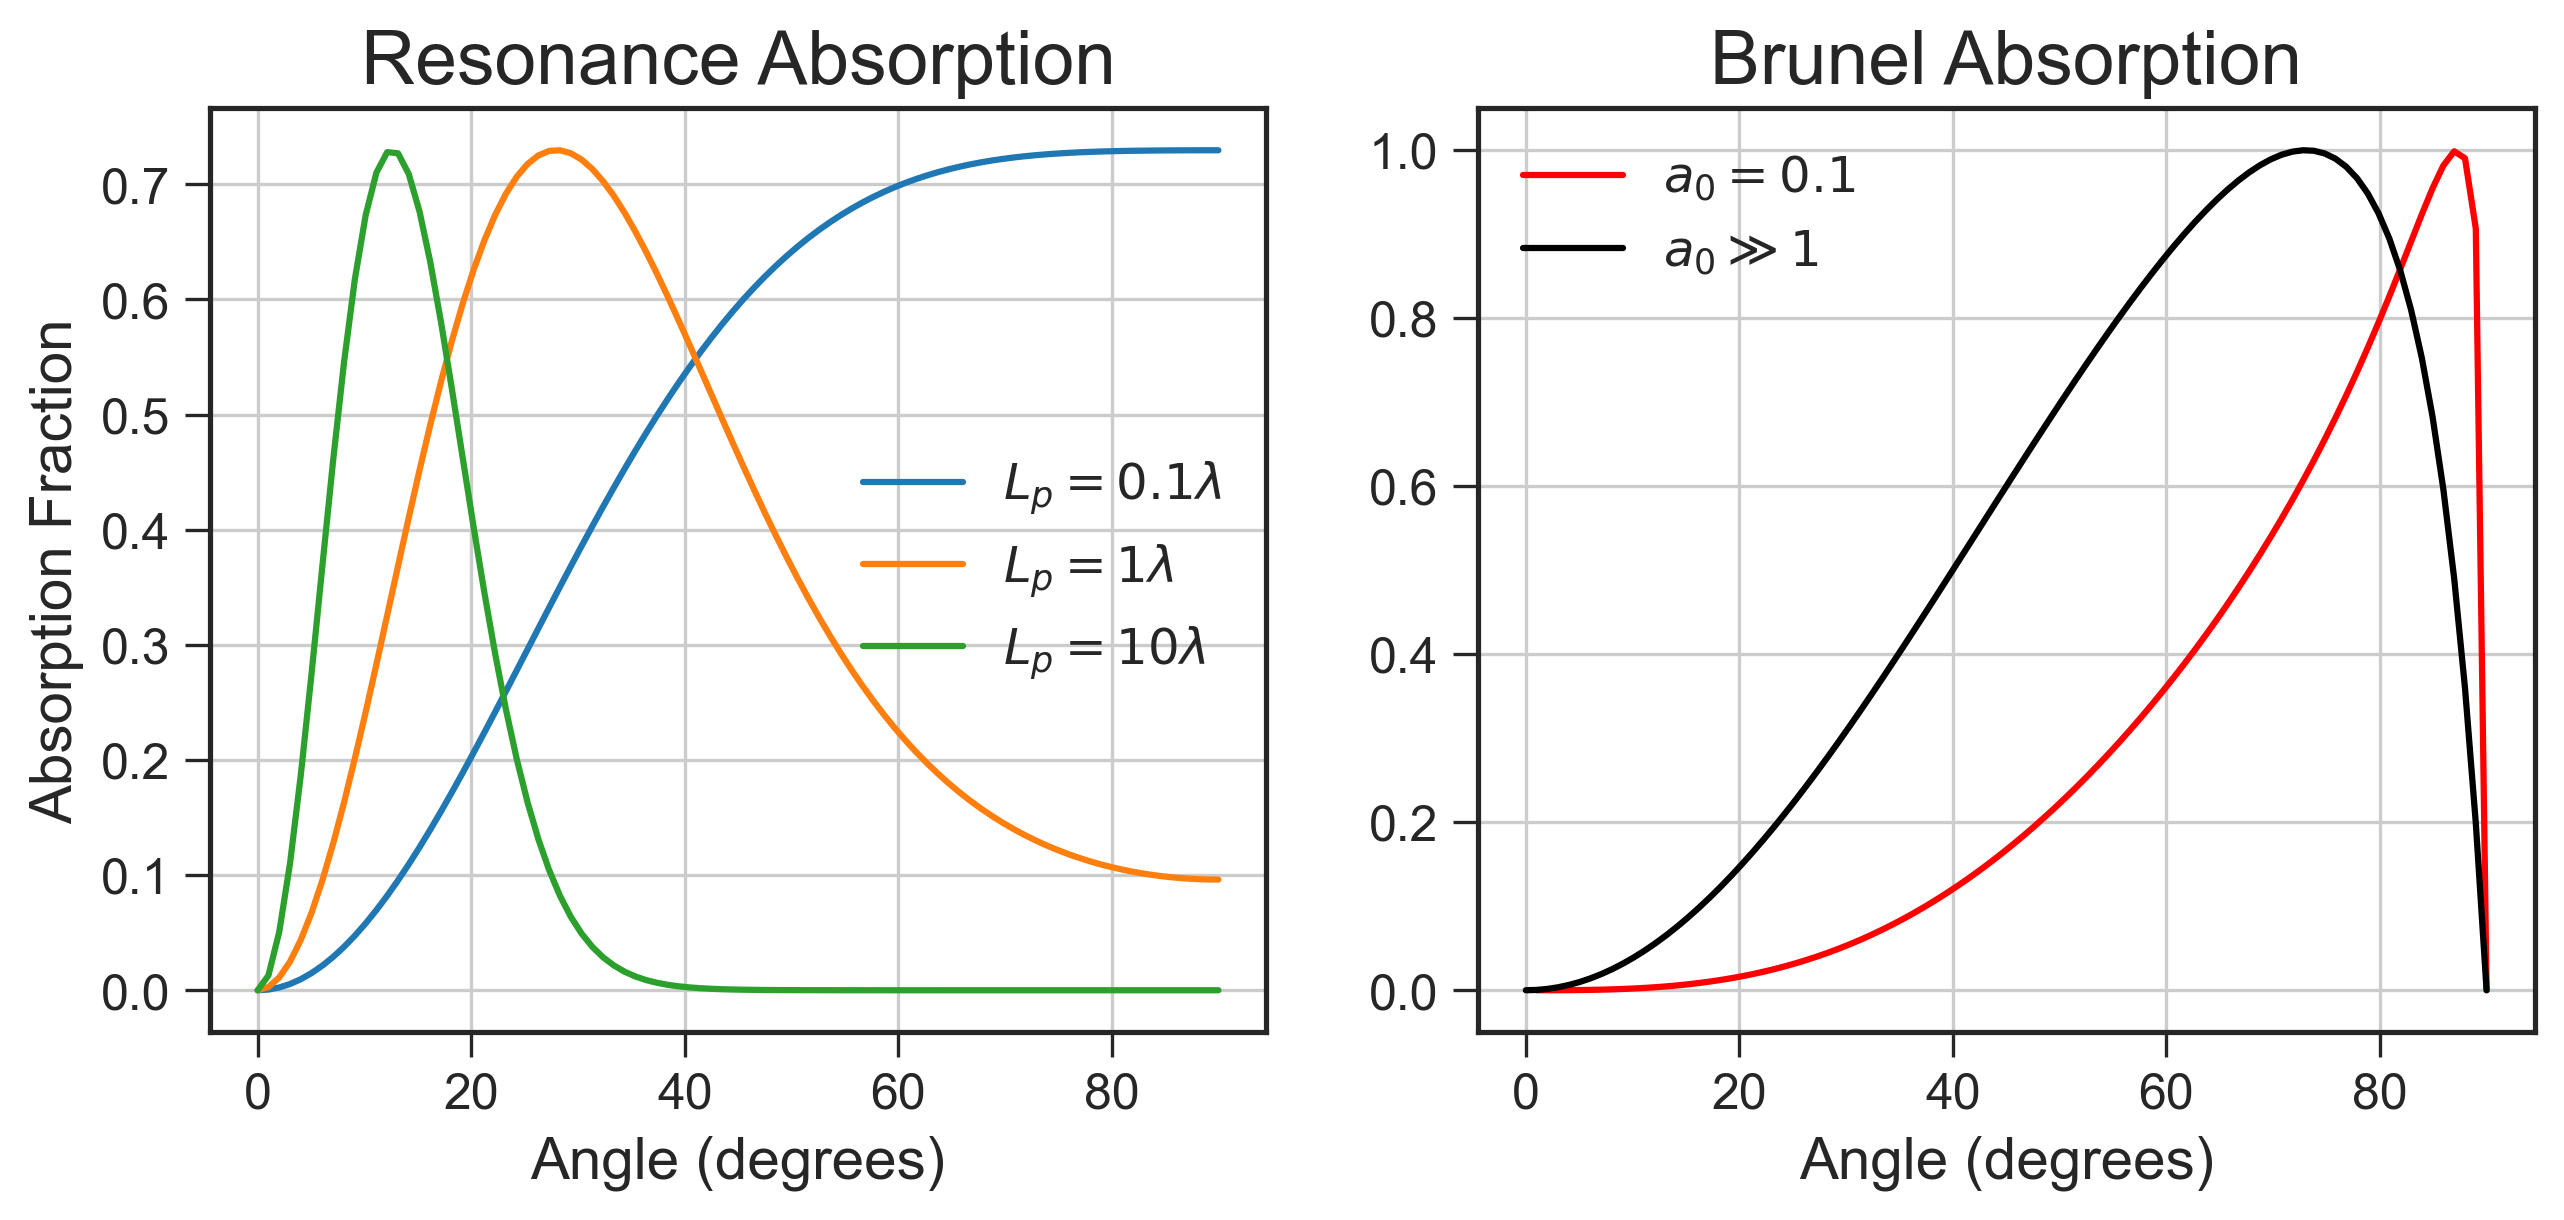
\includegraphics[width=\linewidth]{planning/images/absorption.png}
	\caption{Absorption fraction as a function of incidence angle $\theta_i$. For resonance absorption, the density scale length $L_p$ is varied in terms of the laser wavelength $\lambda = \SI{0.8}{\mu \meter}$. For the Brunel mechanism, fractions are plotted for two regimes $a_0 \ll 1$ (where a value of $a_0 = 0.1$ was chosen) and for $a_0 \gg 1$ (which has no dependence on $a_0$).}
	\label{fig:absorption}
\end{figure}

\subsubsection{Brunel Heating}
Resonance absorption only makes sense when the amplitude of the plasma oscillations $x_\text{osc} = v_\text{osc} / \omega = \frac{a_0 \lambda}{2 \pi}$ is less than the scale length $L_p$ \cite{Gibbon_2005_Plasma}. Otherwise there is not enough available space for the oscillations to take place. For $\lambda = \SI{0.8}{\mu \meter}$ and $a_0 = 1$, $x_\text{osc} = \SI{127}{\nano \meter}$. However, for extremely small scale-lengths, efficient electron heating can still be observed \cite{Grimes_1999_PRL}. Consequently, a different type of heating mechanism is responsible (somewhat confusingly) called ``not so resonant, resonant absorption'' \cite{Brunel_1987_PRL}. This model, developed by Brunel, is also known as \emph{vacuum heating} and will be explained below. 

Before explaining the Brunel mechanism, it is instructive to explain Corkum's 3-step model for \gls{HHG} \cite{Corkum_1993_PRL}\footnote{Readers may find this model more familiar due to the recent 2023 Nobel Physics Prize won by Ohio State's Pierre Agostini \cite{Nobel_2023} which utilized the ideas of this model to produce attosecond pulses}. This model involves a strong oscillating electric field $E(x) = E_0 \cos(\omega t)$ incident on an atom that ionizes an electron at time $t=t^*$. Under the influence of the oscillating field, the (initially stationary) electron will gain  and lose energy by moving away from the atom and returning back toward the atom. When $t^* \neq n \pi$ for integer $n$, it is possible for the electron to return back to the atom with non-zero energy. In fact, when $\omega t^* \approx 17^\circ + n \cdot 180^\circ$, the electron returns with an energy peaking at $3.17 U_p$ where $U_p$ is the ponderomotive potential given by \cref{eq:pond_potential}. Furthermore, modeling the ionization rate through quantum-mechanical tunneling of an electron through a Coulomb potential warped by the oscillating laser field, we also determine that the most probable energy for an electron is strongly peaked at the $3.17 U_p$ cutoff. In short, this model shows how a laser field can produce electrons with energy on the scale of the ponderomotive potential with high probability at a frequency of twice per optical cycle. 

The Brunel mechanism \cite{Brunel_1987_PRL} considers a laser field incident on a planar target at $x > 0$ and vacuum at $x < 0$. In order for the electrons to escape the target, there needs to be some component of the electric field in the $x$ direction. Thus, we need to consider oblique incidence and p-polarization just like with resonance absorption. When the plasma scale length is small, the electrons will be able to travel far enough in the $x < 0$ region to escape the plasma entirely and gain energy on the order of $U_p$ in a similar fashion to Corkum's model \cite{Corkum_1993_PRL}. Electrons returning to the target at just the right time will penetrate deeper than the skin depth $l_s \approx c / \omega_p$ and be inaccessible to the laser field \cite{Gibbon_2005_Plasma}. These \emph{hot electrons}, generated primarily on the front surface of the target, will provide the energy to heat the remainder of the overdense target region that the laser field cannot directly access. 

The optimal angle would appear to be grazing incidence ($\theta_i = 90^\circ$), but Gibbon notes that accounting for imperfect reflection of the laser field and relativistic energies of the electrons, the efficiency no longer diverges at $\theta = 90^\circ$ \cite{Gibbon_2005_Plasma}. In \cref{fig:absorption}, some estimates for the absorption efficiency are plotted according to a simplified model developed by Gibbon \cite{Gibbon_2005_Plasma} based on Brunel \cite{Brunel_1987_PRL}.

\subsubsection{Other Mechanisms}
When the laser field penetrates a distance $l_s \approx c / \omega_p$ into the overdense region of the target, the electrons heat up through collisions at an absorption rate $\eta \propto \frac{\nu_{ei}}{\omega_p,i}$ \cite{Gibbon_2005_Plasma} where $\nu_{ei}$ is the electron-ion collision frequency. This type of absorption is called the \emph{skin effect}. In this case, we see Fresnel-like reflection and absorption \cite{Griffiths_2017} that is effective for large incidence angles. Even when the collision frequency is low, we can still get efficient absorption as long as the thermal electron motions are large compared to the skin depth (i.e. $v_{th}/\omega > l_s$) \cite{Gibbon_2005_Plasma}. This phenomena is called the \emph{anomalous skin effect} that is also most effective at large incidence angles. 

All of the mentioned phenomena work best at oblique incidence in p-polarization. But, for relativistic intensities, additional heating mechanisms arise. When $a_0 \gtrapprox 1$, the magnetic portion of \cref{eq:lorentz} becomes significant. At normal incidence, the electric and magnetic field components both fall in the $y-z$ plane. The electric fields strongly perturb the electrons causing a current $\vec{J}$ that interacts with the laser magnetic field $\vec{B}$ in the direction perpendicular to both. As a result, this type of heating is known as $\vec{J} \times \vec{B}$ heating \cite{Gibbon_2005_Plasma,Kruer_1985_PoF}. Because $\vec{J} \times \vec{B}$ is in the direction of propagation, this effect is most pronounced at normal incidence.

At even higher intensities, the laser can directly impart energy to the electrons through radiation pressure \cite{Macchi_2013_RevModPhys} because photons carry momentum. These mechanisms are explored further in \cref{sec:acceleration}. In reality, all experiments involve a combination of several different electron heating mechanisms. Consequently, many experiments and simulations have been devoted to parametric studies that show how parameters ($L_p$, $\theta_i$, polarization, $a_0$, etc.) affect electron absorption \cite{Sheng_2015_CPB}.

\section{Ion Acceleration} \label{sec:acceleration}

The previous section gave an overview of the laser-plasma interactions and how they can efficiently couple energy into hot electrons. Regardless of heating mechanism, one theme is common to all -- the energy gained by an electron's quiver motion in an oscillatory field, known as the ponderomotive potential (\cref{eq:pond_potential}) sets the scale for the hot electron temperature $T_h$. That equation was only valid for non-relativistic electrons, so we must replace $U_p = \frac{1}{4} m v_\text{osc}^2$ with the relativistic energy $U_p \equiv (\gamma - 1) m c^2$ where $\gamma = 1 / \sqrt{1 - \frac{v_\text{osc}^2}{c^2}}$ defines the lorentz factor. We can combine this with the relativistic momentum $p = \gamma m v_\text{osc}$ and \cref{eq:a0} to determine an approximate expression of $\gamma$ in terms of $a_0$
	
\begin{equation}
	\gamma \simeq \sqrt{1 + a_0^2} = \sqrt{1 + \frac{I_{18} \lambda_{\mu m}^2}{1.37}} \label{eq:gamma}
\end{equation}
where $I_{18}$ is the peak intensity of the laser pulse in $10^{18}$ $\unit{\watt \per \centi \meter \squared}$ and $\lambda_{\mu m}$ is the wavelength in $\mu$m. In 1992, Wilks \cite{Wilks_1992_PRL} conducted simulations to show that $T_h$ is on the order of $U_p$. 

\begin{equation}
	k_B T_h \approx m c^2 (\gamma - 1) \label{eq:wilks}
\end{equation}
In \autoref{fig:electron_scaling}, we can see that the \emph{Wilks scaling} (pink) closely matches ultra-intense laser experiments. The other scalings in the figure are similarly validated by computational simulations and are all proportional to $(I \lambda^2)^\alpha$, where $0 < \alpha \leq 1$. As a result, the product $I \lambda^2$ is an important quantity in laser-plasma experiments and is called the \emph{irradiance}. Wilks also outlines a way to measure the hot electron temperature in his simulations \cite{Wilks_1992_PRL} by taking the slope of $\frac{dN_e}{dE}$ in the MeV regime\footnote{For example, the slopes in \autoref{fig:sim_spectrum}(b) yield a $T_h$ between 2 and 3 MeV}.

\begin{figure}
	\centering 
	\includegraphics[width=0.75\linewidth]{planning/images/gibbon_hot_electron.PNG}
	\caption{Experimentally recorded hot electron temperatures as a function of irradiance $I \lambda^2$ are plotted as red squares. The empirical scaling models are given by Wilks \cite{Wilks_1992_PRL}(pink, solid), Gibbon and Bell \cite{Gibbon_1992_PRL}(blue, ashed), Forslund et. al. \cite{Forslund_1977_PRL}(green, dash-dot), and Brunel \cite{Brunel_1987_PRL}(black, dotted). Figure is taken from Gibbon \cite{Gibbon_2005_Plasma}}
	\label{fig:electron_scaling}
\end{figure}
Since protons are 1836 times as massive as electrons, they are much harder to accelerate and (on the scale of femtosecond pulse interactions) are essentially immobile. Despite this, ultra-intense laser experiments have demonstrated proton acceleration is possible. This section will explain the \gls{TNSA} mechanism for accelerating protons and light ions which is heavily dependent on $T_h$. Then, we will discuss alternative acceleration mechanisms. Finally, we'll overview some important applications.

\subsection{Target Normal Sheath Acceleration}
The observation of energetic protons off the rear side of thin plastic and gold targets has been documented throughout a variety of experiments since the 80s \cite{Tan_1984_PoF}. It might sound unintuitive that we would even see protons in the first place; after all, when shooting a target like aluminum, one would expect aluminum ions. It turns out that there is always an important and measurable surface contamination layer, primarily composed of hydrogen and light hydrocarbons \cite{Gitomer_1986_PoF}. Allen \cite{Allen_2004_PRL} showed that when removing the surface contaminant from the backside, we see a strong suppression in ion acceleration. This points to the contaminant layer being the crux of what is accelerated.

\subsubsection{TNSA Models}

Expansion models have been long known since the 70s and 80s \cite{Crow_1975_JPP,Kishimoto_1983_PoF} that describe the acceleration of protons with experiments (e.g. Tan \cite{Tan_1984_PoF}) as well. However, \gls{CPA} \cite{Strickland_1985_Optics} allowed the laser peak intensities to reach relativistic levels ($a_0 > 1$) with sub-ps pulse duration as explained in \autoref{sec:lasers}.

The first \gls{TNSA} experiment occurred in 2000 with a group at Michigan \cite{Maksimchuk_2000_PRL}. They found 1.6 MeV protons from a thin aluminum foil with a $\SI{3e18}{\watt \per \centi \meter \squared}$ class laser at normal incidence. Then, \gls{RAL} found 30 MeV protons \cite{Clark_2000_PRL} from a $\SI{5e19}{\watt \per \centi \meter \squared}$ class laser incident on a lead target at $45^\circ$ incidence. Shortly after, \gls{LLNL} found energies up to 58 MeV \cite{Snavely_2000_PRL} from a $\SI{3e20}{\watt \per \centi \meter \squared}$ class laser on a gold target at $45^\circ$ incidence.

With efficient MeV proton acceleration demonstrated through multiple studies, a more comprehensive picture of the process emerged. In 2001, Wilks \cite{Wilks_2001_PoP} summarized much of the existing literature including the isothermal expansion model \cite{Crow_1975_JPP}, existence of a maximum cutoff energy \cite{Kishimoto_1983_PoF}, and dependence on hot temperature \cite{Wilks_1992_PRL}. Then, he described the \gls{TNSA} process in the following way \cite{Wilks_2001_PoP}

\begin{quote}
	... the prepulse creates large plasma in front of a solid target. Once the main pulse hits the target, a cloud of energetic electrons (1-10 MeV in effective temperature) is generated, which extends past the ions on both the front and back of the target. Since the protons on the back are in a sharp, flat density gradient, they are accelerated quickly (in the first few $\mu m$ off the target) to high energies in the forward direction ... On the front, the outermost ions are in a sphere, in a long scale length plasma (due to prepulse) and therefore are accelerated to lower energies, and are spread out into $2 \pi$ steradians.
\end{quote}

\begin{figure}
	\centering 
	\includegraphics[width=\linewidth]{planning/images/tnsa.PNG}
	\caption{The target normal sheath acceleration process is depicted. First, an intense laser pulse irradiates the front side of a target foil of few $\mu m$ thickness. This generates hot electrons that stream through the foil and re-emerge in a cloud on the rear side. The charge separation of the hot electrons and positively charged target creates intense longitudinal fields ($\sim$ TV/m) that accelerate light ions in the mostly target normal direction. This figure was taken from Roth \cite{Roth_2016_CERN_TNSA}}
	\label{fig:tnsa}
\end{figure}
A visual of the \gls{TNSA} process can be seen in \cref{fig:tnsa}. Although Wilks \cite{Wilks_2001_PoP} provided a physical picture of the \gls{TNSA} process, existing models did not always match up to experiments. For this reason, the ensuing decade saw much progress in the development of models to describe the spectrum of \gls{TNSA} accelerated protons. Perego \cite{Perego_2011_NIaMiP} provides a good review of some of the leading models developed and tested against experiments in the 2000s and these models will be summarized below. 

First, are the isothermal expansion (fluid) models which include Mora's ``Plasma Expansion into a Vacuum'' \cite{Mora_2003_PRL} (2003) that combine Equations \eqref{eq:poisson} and \eqref{eq:boltzmann} with fluid Equations \eqref{eq:continuity} and \eqref{eq:lorentz_mora}. This model underlies the work done in \cref{ch:5}, where it is explained in more detail, and has the issue of predicting proton energies that can go up to arbitrarily high values. As a remedy, Mora introduces a finite acceleration time $\tau$ which is of the order of the pulse duration. Mora \cite{Mora_2005_PRE} addresses this in a different way (2005) by instead assuming an adiabatic model and limiting the target to be a thin foil (instead of a semi-infinite target). 

Alternatively, Passoni and Lontano \cite{Passoni_2004_LaPB} introduces an upper limit to the integration range of the electric potential instead of using the fluid equations. In this approach, the electric fields determined from the potential are considered static, and the ensuing ion dynamics is determined by placing a test ion in the field. Further iterations incorporate some distribution of speeds for the electrons (non-relativistic Maxwell-Boltzmann \cite{Lontano_2006_PoP} or relativistic Maxwell-Juttner \cite{Passoni_2008_PRL}) and use an empirically determined scaling for the peak energy of electrons (as a function of laser energy) that do not escape the system \cite{Perego_2012_RevSci}.

Furthermore, some hybrid models include elements of both fluid and quasistatic models like Robinson \cite{Robinson_2006_PRL} and Albright \cite{Albright_2006_PRL}.

\subsubsection{Optimization of TNSA process} \label{sec:tnsa_opt}

Since the \gls{TNSA} process is intimately related to hot electron generation at the front of the target and a flat density gradient at the back, many efforts have been taken to design targets that optimize ion acceleration. Patel \cite{Patel_2003_PRL} used spherically shaped targets to act as a lens that focus the proton beam. MacKinnon \cite{Mackinnon_2002_PRL} showed lower target thickness leads to higher proton energy due to a higher mean density of hot electrons at the surface. More recent experiments have even used nanowires \cite{Vallieres_2021_Nature} and microtubes \cite{Strehlow_2022_Nature}. Many experiments generally find that there is an optimal level of pre-expansion of the target that enhances hot electron generation and ion acceleration (e.g. McKenna \cite{McKenna_2008_LaPB}).

Another way to increase the peak proton energy of the emitted spectrum is to use two spatially aligned pulses. If one pulse has a delay with respect to the other, the first pulse could pre-expand the target to provide an optimal electron density at the front surface \cite{Ferri_2018_PoP}. If the pulses are also temporally aligned, the constructive interfere at the target front surface may prove beneficial \cite{Ferri_2019_Nat_Comm}. The second approach is called double pulse enhanced \gls{TNSA} and \cref{ch:4} is devoted to this phenomenon. 

See the review article by Roth \cite{Roth_2016_CERN_TNSA} for a more comprehensive list of the different approaches to enhance TNSA.

\subsection{Other Acceleration Mechanisms}
\gls{TNSA} is not the only method in which protons can be accelerated. For intensities of greater than $10^{21} \text{ W cm}^{-2}$, laser-induced ion shocks can start to play a significant role \cite{Fuchs_2005_Nat}. For even higher intensities $\sim 10^{23} \text{ W cm}^{-2}$, the radiation pressure of electromagnetic waves can efficiently transfer momentum to ions \cite{Fuchs_2005_Nat}. See Macchi \cite{Macchi_2013_RevModPhys} for a more in depth discussion on these topics. One way to differentiate the \gls{TNSA} regime from other regimes is through the following equation relating $a_0$ to various properties of the laser and target

\begin{equation}
	a_0 = n_e \lambda r_e l_0 = 224 \left(\frac{n_e}{\SI{1e29}{\per \meter \cubed}}\right) \left(\frac{l_0}{\SI{1}{\micro \meter}} \right) \label{eq:acc_regime}
\end{equation}
Lezhnin \cite{Lezhnin_2015_PoP} uses this equation as a dividing line to differentiate \gls{TNSA} from two other mechanisms: \gls{RPA} and Coulomb Explosions; this can be seen in \autoref{fig:regimes}. If the laser intensity is sufficiently high and density is low enough to be transparent, the laser can quickly sweep away most electrons to leave behind a strongly positive target. The repelling coulomb force will cause the protons to expand outwards in all directions.

When the radiation pressure $P_\text{rad} \approx 2 I_0 / c$ is significant enough to overcome the thermal expanding pressure $n_e k_B T_e$, ions can accelerate directly through the transfer of momentum. \cite{Macchi_2013_RevModPhys}. In this regime, laser absorption into hot electrons by traditional mechanisms would be detrimental. By shooting the laser at normal incidence with circular polarization, resonance absorption and $\vec{J} \times \vec{B}$ heating can be minimized as seen in \autoref{sec:absorption}.

For thick targets, this immense pressure can impart a parabolic deformation that allows the laser to penetrate further. This is the regime of \emph{hole boring}. Targets thin enough where the hole boring process reaches the target rear in a time less than the pulse duration are in the \emph{light sail} regime. \cite{Macchi_2013_RevModPhys}. 

\begin{figure}
	\centering 
	\includegraphics[width=0.75\linewidth]{planning/images/acceleration_regimes.PNG}
	\caption{The regimes of three different acceleration mechanisms are displayed in terms of \cref{eq:acc_regime}. This figure was taken from Roth \cite{Lezhnin_2015_PoP}}
	\label{fig:regimes}
\end{figure}

\subsubsection{Wakefield Acceleration}
All the aformentioned acceleration processes only make sense for overdense targets whose electron density is greater than the critical density ($n_e > n_c$). This is because the critical density surface is the primary area where the laser deposits energy into hot electrons. If the target plasma has $n_e < n_c$, the target is said to be underdense and there is no critical density surface where the laser interacts with. Tajima and Dawson \cite{Tajima_1979_PRL} first proposed the idea of a ``Laser Electron Accelerator'' in 1979 that is capable of accelerating electrons to high energies through the non-linear ponderomotive force. If the conditions are just right, the electrons can ``surf'' a plasma wave in the wake of the pulse and pull along positive ions in a process now known as \gls{LWFA}. A comprehensive review of the subject can be found here \cite{Esarey_2009_LPA}.

%\subsection{Notes}
%
%should talk about Bragg Peak and how that works based on coulomb collision
%
%E = kT / e L where L is related to the debye length or scale length
%
%Heavy ions stay still, hot electrons expand out several debye lengths: causes charge separation that accelerates light ions/protons. Characteristic: accelerated in the normal direction even though laser is at oblique incidence. High scale reduces TNSA electric field b/c boundaries are not as sharp on the backside (to make a capacitor like field). 
%
%Spectrum of TNSA beams is typically broadband up to a cutoff energy. The dN/dE looks kind of thermal i.e. exponentially decaying.  
%
%Also, a sharp angular boundary in the proton angular distribution (clearer in higher Z and thicker targets) is consistent with a bell-shaped transverse distribution of hot electrons in the rear surface sheath due to the fact that the density will naturally be higher along the laser axis and decreases with transverse radius. 
%
%Then, they talk about TNSA modeling which I've already covered: Passoni, Mora, etc.
%
%Can look at Joe Smith's TNSA experiment paper (is it on arxiv?) to see better evidence of the relationships and how they fare with experiments.
%
%Can give a simple estimate of the regime it is relevant by considering intensities where we get relativistic ions. However, this is really, really high and thus why we consider TNSA as the dominant mechanism. We don't have lasers this high of an intensity for these affects to be relevant, so it must come from TNSA i.e. strong electrostatic fields from electrons rather than direct electron acceleration.
%
%Then, in the relativistic transparency regime of thin targets, the laser pulse can actually deposit well into the target. Of course, this means that the laser isn't pushing on the front edge of the target so that we aren't in the RPA regime anymore. In this regime, the Breakout afterburner (BOA) model is typically employed. 
%
%Finally collisionless shock acceleration (CSA) becomes relevant when shocks appear and ions reflect off this shock front with speed $2 v_s$ where $v_s = M c_s$ and $M > 1$ is the Mach number. \citep{Fiuza_2013_PoP} talks about how shock acceleration is optimal for near critical density targets that particularly have an exponential scale length plasma on the rear side of $L_g \approx \lambda_0 / 2 \sqrt{m_i/m_e}$ for uniform electron heating and ion reflection. They also say that the target should be thin enough so that $L < 2 \pi c / \omega_{p,i}$ but not too much smaller. 
